% !TEX root = main.tex

%%%%%%%%%%%%%%%%%%%%%%%%%%%%%%%%%%%%%%%%%%%%%%%%%%%%%%%%%%%%%%%%%%%%%%%%%%%%%%%%%%%%%%%%%%%%%%%%
\section{結果}
%%%%%%%%%%%%%%%%%%%%%%%%%%%%%%%%%%%%%%%%%%%%%%%%%%%%%%%%%%%%%%%%%%%%%%%%%%%%%%%%%%%%%%%%%%%%%%%%

\subsection{実験課題1}
ソレノイド底面を$z=0\,[\si{cm}]$とし,各$z$座標における測定結果を以下の
図5~図23に示す.また,$z$座標と磁気プローブの出力$V_{c0}$の積分である
$\int_{0}^{t}V_{c0}(t)dt$との測定結果を表1に示す.
ただし,磁気プローブの出力$V_{c0}$の積分はオシロスコープから得られるデジタルデータ
(テキストデータ)を使用して算出する方法を用いる.

\begin{figure}[H]
    \centering
    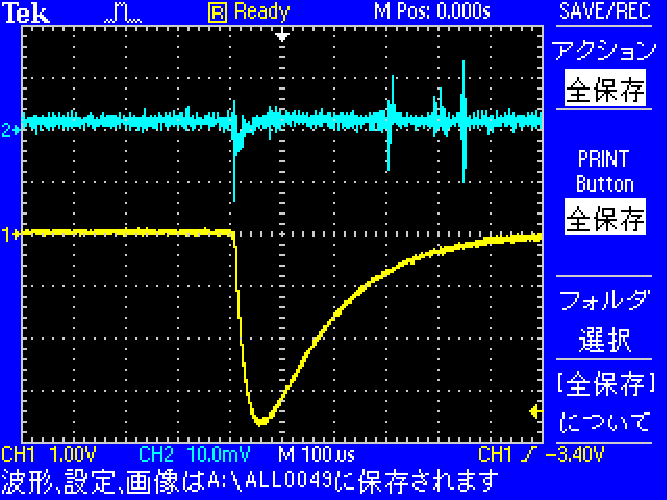
\includegraphics[scale=0.5]{images-23.pdf}
    \caption{$z=-10\,[cm]$における測定結果}
\end{figure}

\begin{figure}[H]
    \centering
    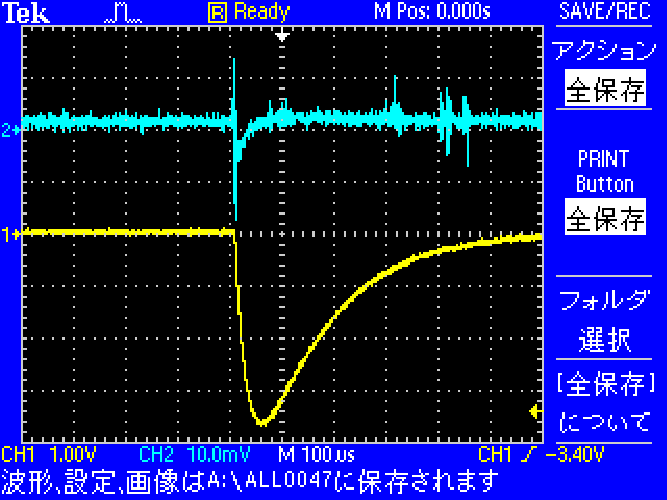
\includegraphics[scale=0.5]{images-22.pdf}
    \caption{$z=-8\,[cm]$における測定結果}
\end{figure}

\begin{figure}[H]
    \centering
    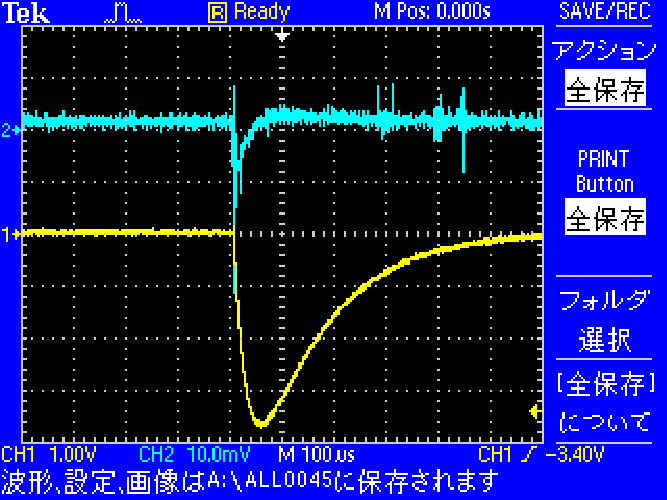
\includegraphics[scale=0.5]{images-21.pdf}
    \caption{$z=-6\,[cm]$における測定結果}
\end{figure}

\begin{figure}[H]
    \centering
    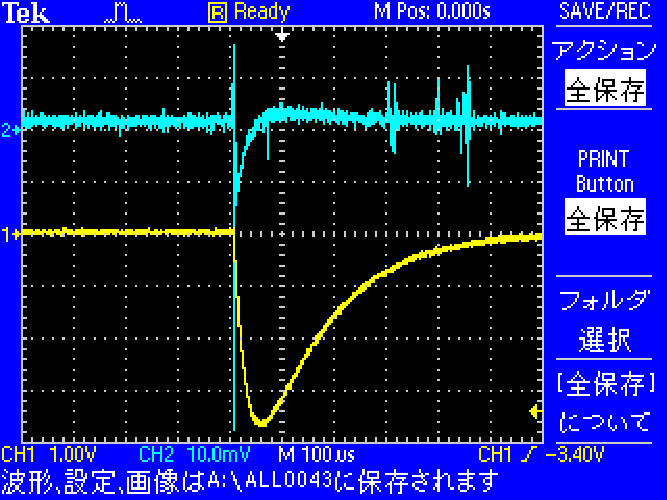
\includegraphics[scale=0.5]{images-20.pdf}
    \caption{$z=-4\,[cm]$における測定結果}
\end{figure}

\begin{figure}[H]
    \centering
    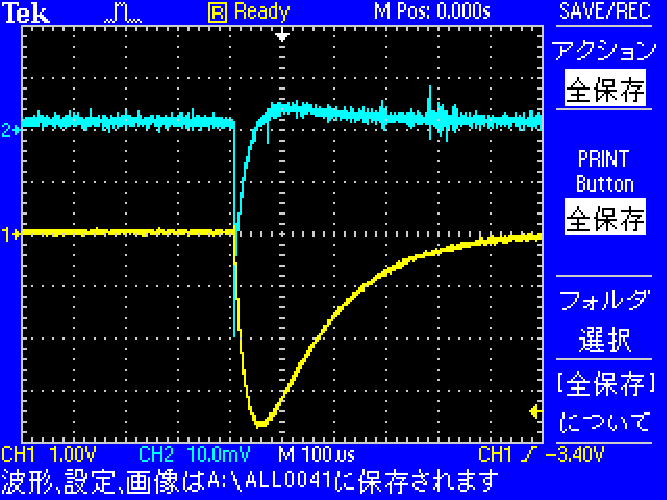
\includegraphics[scale=0.5]{images-19.pdf}
    \caption{$z=-2\,[cm]$における測定結果}
\end{figure}

\begin{figure}[H]
    \centering
    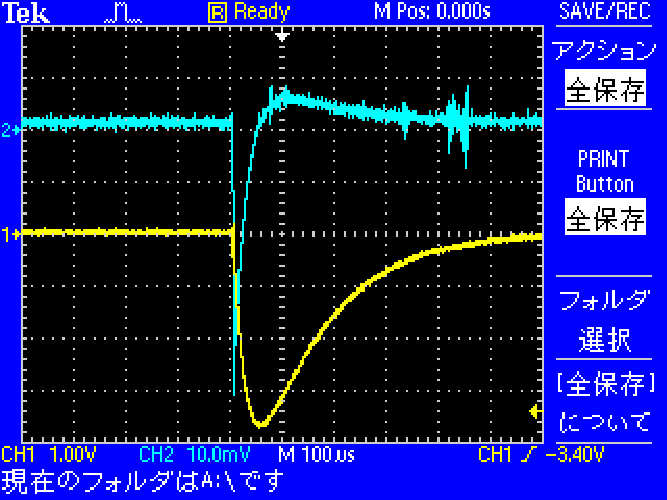
\includegraphics[scale=0.5]{images-1.pdf}
    \caption{$z=0\,[cm]$における測定結果}
\end{figure}

\begin{figure}[H]
    \centering
    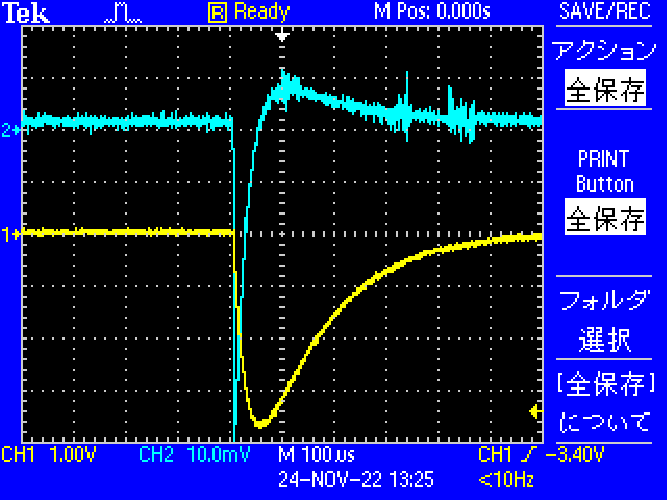
\includegraphics[scale=0.5]{images-2.pdf}
    \caption{$z=2\,[cm]$における測定結果}
\end{figure}

\begin{figure}[H]
    \centering
    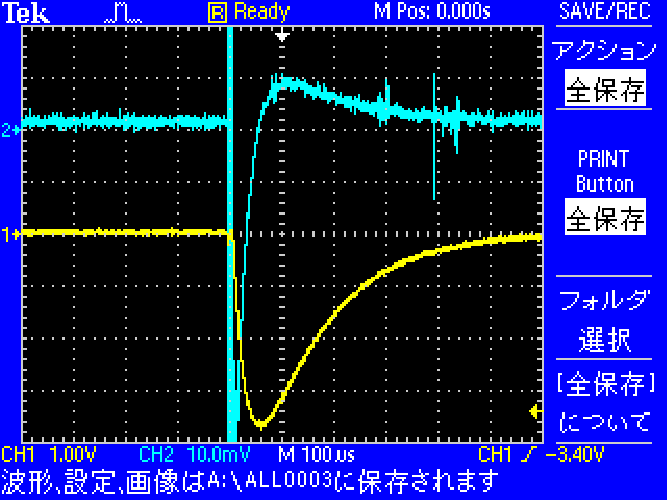
\includegraphics[scale=0.5]{images-3.pdf}
    \caption{$z=4\,[cm]$における測定結果}
\end{figure}

\begin{figure}[H]
    \centering
    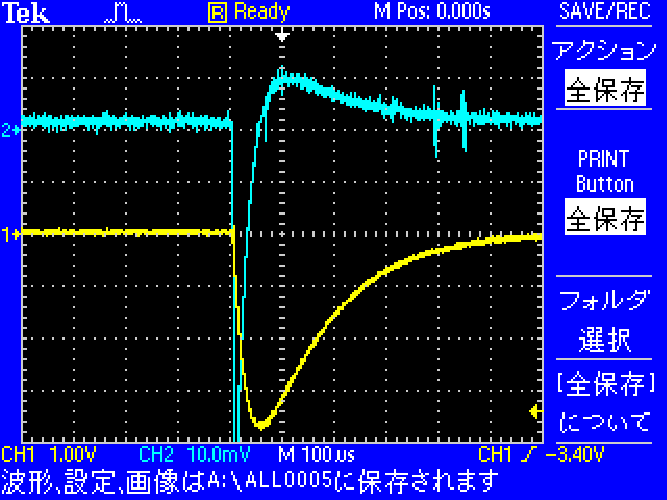
\includegraphics[scale=0.5]{images-4.pdf}
    \caption{$z=6\,[cm]$における測定結果}
\end{figure}

\begin{figure}[H]
    \centering
    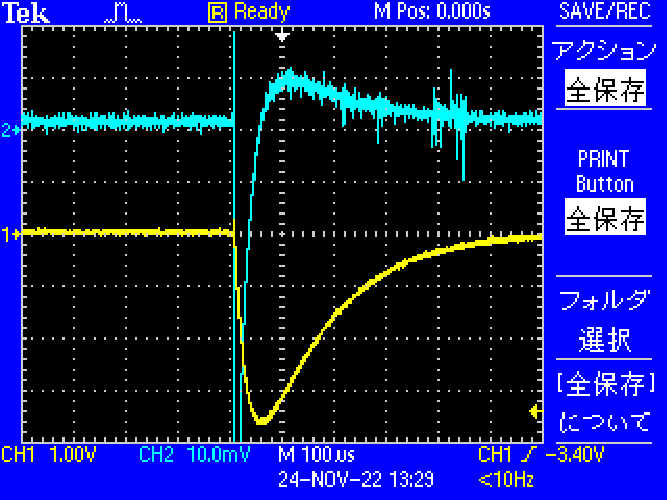
\includegraphics[scale=0.5]{images-5.pdf}
    \caption{$z=8\,[cm]$における測定結果}
\end{figure}

\begin{figure}[H]
    \centering
    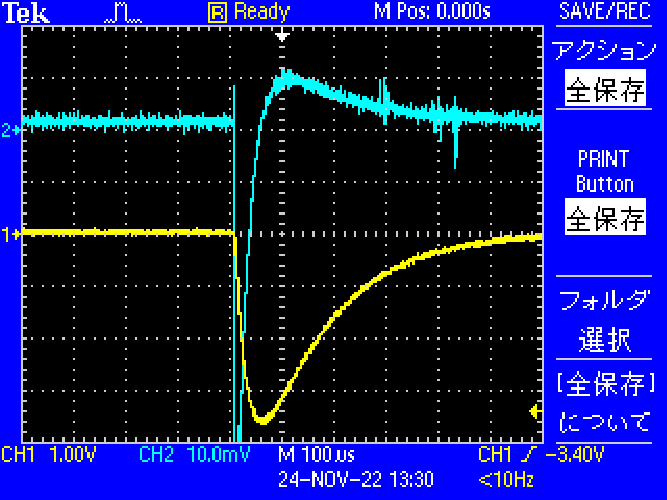
\includegraphics[scale=0.5]{images-6.pdf}
    \caption{$z=10\,[cm]$における測定結果}
\end{figure}

\begin{figure}[H]
    \centering
    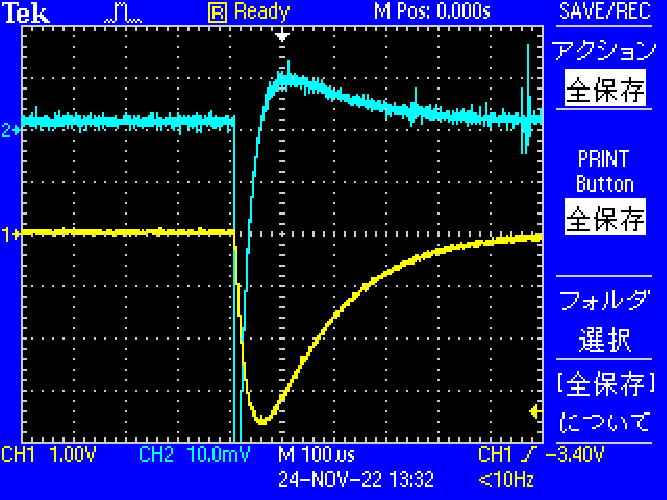
\includegraphics[scale=0.5]{images-7.pdf}
    \caption{$z=12\,[cm]$における測定結果}
\end{figure}

\begin{figure}[H]
    \centering
    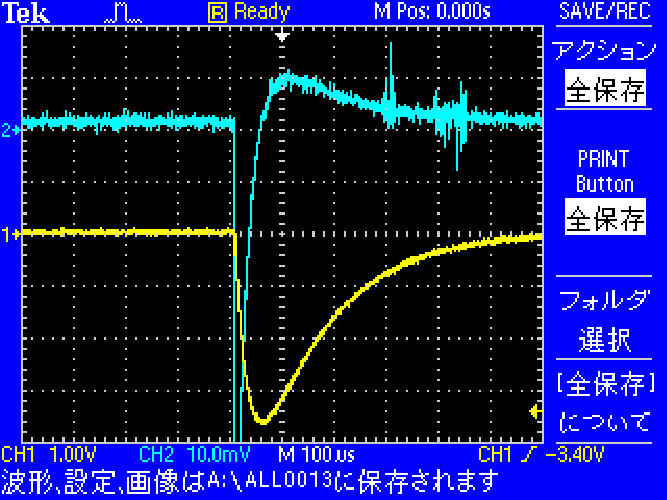
\includegraphics[scale=0.5]{images-8.pdf}
    \caption{$z=14\,[cm]$における測定結果}
\end{figure}

\begin{figure}[H]
    \centering
    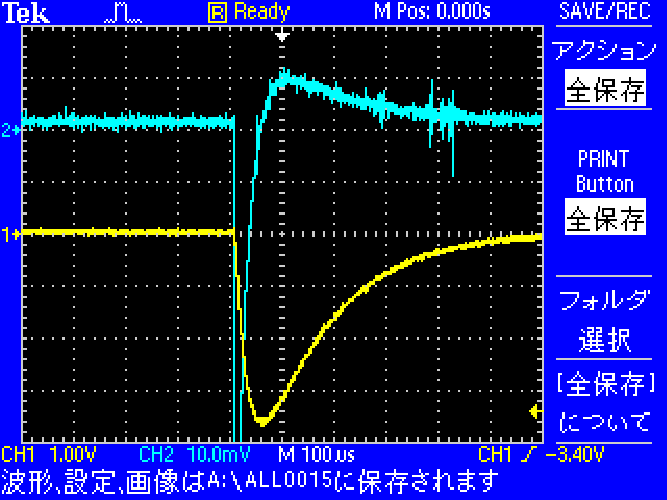
\includegraphics[scale=0.5]{images-9.pdf}
    \caption{$z=16\,[cm]$における測定結果}
\end{figure}

\begin{figure}[H]
    \centering
    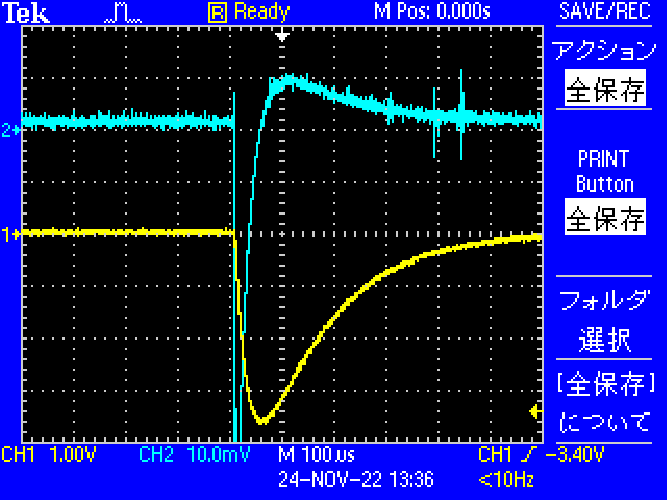
\includegraphics[scale=0.5]{images-10.pdf}
    \caption{$z=18\,[cm]$における測定結果}
\end{figure}

\begin{figure}[H]
    \centering
    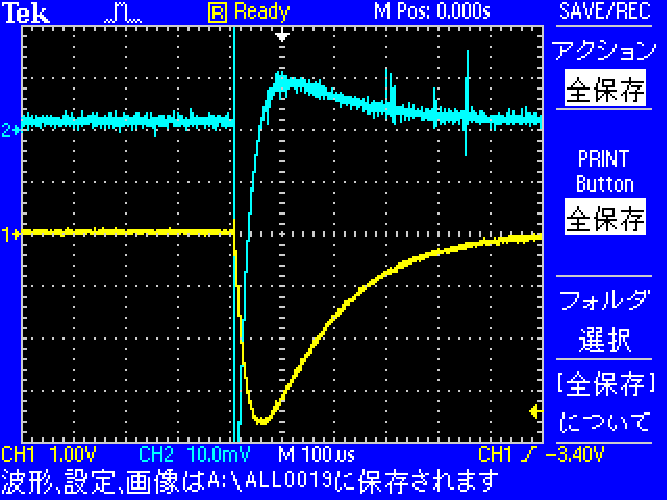
\includegraphics[scale=0.5]{images-11.pdf}
    \caption{$z=20\,[cm]$における測定結果}
\end{figure}

\begin{figure}[H]
    \centering
    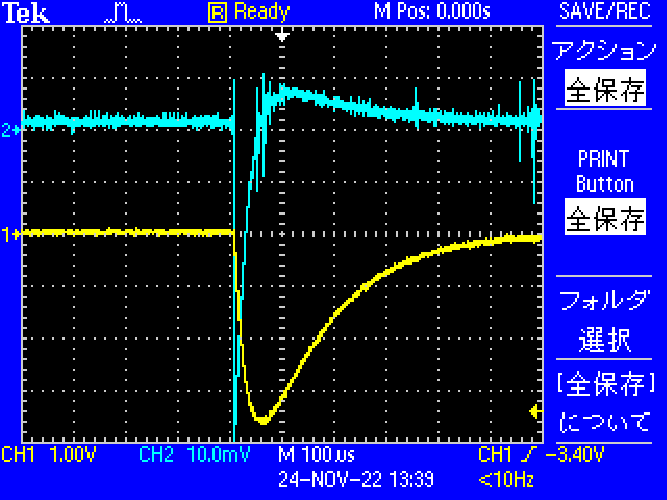
\includegraphics[scale=0.5]{images-12.pdf}
    \caption{$z=22\,[cm]$における測定結果}
\end{figure}

\begin{figure}[H]
    \centering
    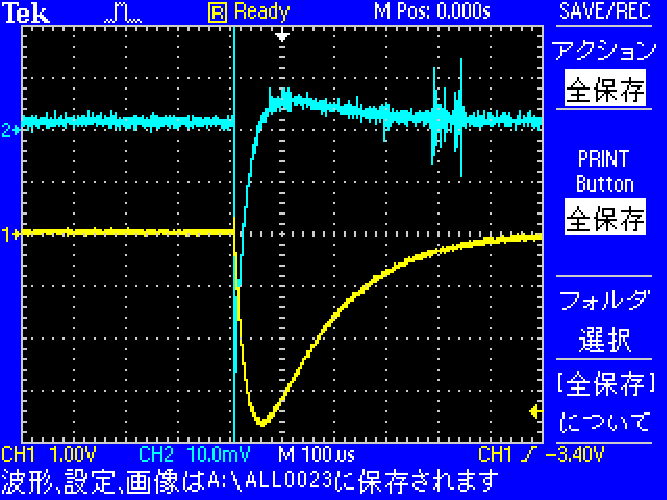
\includegraphics[scale=0.5]{images-13.pdf}
    \caption{$z=24\,[cm]$における測定結果}
\end{figure}

\begin{figure}[H]
    \centering
    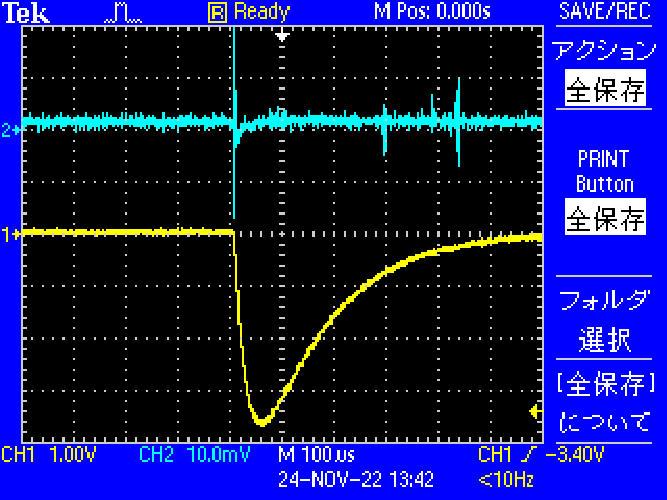
\includegraphics[scale=0.5]{images-14.pdf}
    \caption{$z=26\,[cm]$における測定結果}
\end{figure}

\begin{figure}[H]
    \centering
    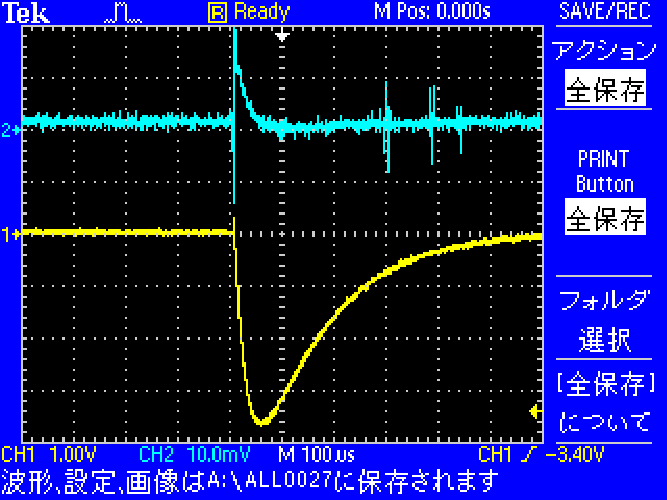
\includegraphics[scale=0.5]{images-15.pdf}
    \caption{$z=28\,[cm]$における測定結果}
\end{figure}

\begin{figure}[H]
    \centering
    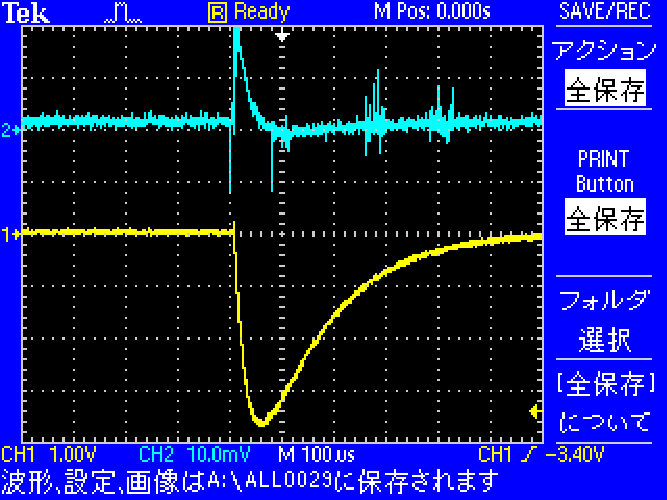
\includegraphics[scale=0.5]{images-16.pdf}
    \caption{$z=30\,[cm]$における測定結果}
\end{figure}

\begin{figure}[H]
    \centering
    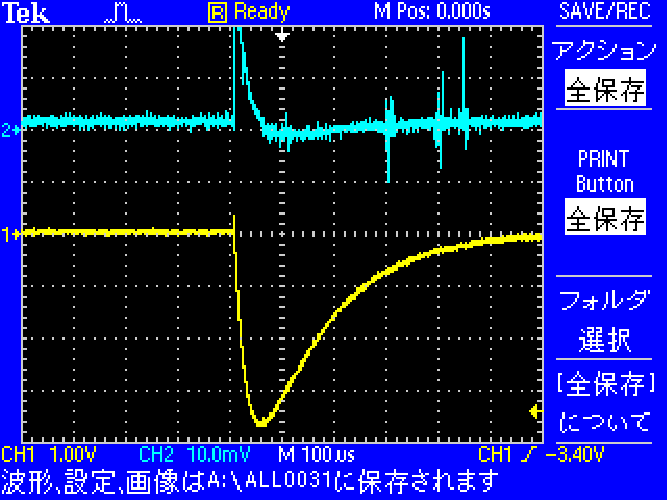
\includegraphics[scale=0.5]{images-17.pdf}
    \caption{$z=32\,[cm]$における測定結果}
\end{figure}

\begin{figure}[H]
    \centering
    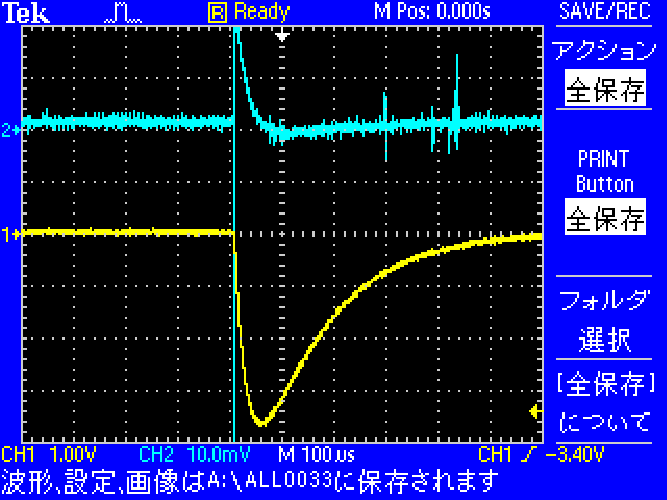
\includegraphics[scale=0.5]{images-18.pdf}
    \caption{$z=34\,[cm]$における測定結果}
\end{figure}